% This file is meant to be included in another 
\documentclass{article}
\usepackage{epsfig}
\begin{document}
\section{{\tt Window()}}

\subsection{Purpose}

Creates vector structure containing a window (also called
a taper, lag window, or apodization function).  The choices
currently available are:
\begin{itemize}
\item Rectangular
\item Hann
\item Welch
\item Bartlett
\item Parzen
\item Papoulis
\item Hamming
\end{itemize}
It should be straighforward to add additional window functions if
they are desired.

\subsection{Synopsis}

% Syntax: argument definitions, calling signature

\begin{verbatim}
#include "Window.h"
#include "AVFactories.h"

void Window (Status *,REAL4Vector *, WindowParams *);

typedef struct tagWindowParams {
  INT4        length;       /* length of window (input) */
  WindowType  type;         /* type of window (input) */
  REAL8       sumofsquares; /* sum of window squared  (ouput) */
  CHAR*       windowname;   /* pointer to a char string with window name (output) */
} WindowParams;

typedef enum {Rectangular,
              Hann,
              Welch,
              Bartlett,
              Parzen,
              Papoulis,
              Hamming} WindowType;

\end{verbatim}
\subsection{Description}

This function creates a window function of the specified type, in the
output vector.

\subsection{Operating Instructions}

% Detailed usage 

\begin{verbatim}
Status status; 
REAL4Vector *vector=NULL;
WindowParams params;

  params.type=Hann;
  params.length=1024;
  CreateVector(&status,&vector,1024);
  Window(&status,vector,&params);
  DestroyVector(&status,&vector);

\end{verbatim}

Note that the {\tt Window()} function sets the fields {\tt params.windowname} and
{\tt params.sumofsquares}.

\subsubsection{Arguments}

% Describe meaning of each argument

\begin{itemize}
\item {\tt status\/} is a universal status strucure. Its contents are 
assigned by {\tt CreateVector}.
\item {\tt vector\/} After
return from {\tt Window()}, {\tt vector} points to a vector containing the window function.
The vector's length must
agree with {\tt params.length} or an error will occur.
\item {\tt params\/} is a structure specifying the type of the window
and containing useful information on return.  The window type {\tt
params.type} and length {\tt params.length} must be set before calling
{\tt Window()}.  On return {\tt params.sumofsquares} is set to the sum of
the squares of the window function, and {\tt params.windowname} points
to a static string containing one-word the window name (for example,
``Parzen").
\end{itemize}

\subsubsection{Options}

The window type and the window length are both required.

\subsubsection{Error conditions}

% What constitutes an error condition? What do the error codes mean?

{\tt Window\/}
sets the universal status structure on return. Non-zero status codes
indicate an error condition. Error conditions are described in
table \ref{tbl:WI}.

\begin{table}
\hskip -0.7in
\begin{tabular}{|r|l|l|}\hline
status&status&Description\\
code&description&\\\hline
WINDOW\_NULLPARAM&$*${\tt params} NULL&must point to a parameter structure\\
WINDOW\_NULLVECTOR&CreateVector() failed&CreateVector() produced null vector\\
WINDOW\_EALLOCATE&CreateVector() failed &CreateVector() failed\\
WINDOW\_ELENGTH&{\tt params.length}$\le 0$&window length must be positive\\
WINDOW\_TYPEUNKNOWN&Unknown window type&Rectangular$\le${\tt params.type}$\le$Hamming\\
WINDOW\_NULLHANDLE&{\tt *vector NULL}&Vector handle is null\\
WINDOW\_WRONGLENGTH&{\tt (*vector)$\rightarrow$length!=params.length}&Vector length incorrect\\
WINDOW\_MSGNULLDATA&{\tt (*vector)$\rightarrow$data==NULL}&input vector data pointer null\\
\hline
\end{tabular}
\caption{Error conditions for {\tt Window()}}\label{tbl:WI}
\end{table}

                                
\subsection{Algorithms}

The window functions are defined for $j=0,\cdots,N-1$ by the following formulae.
In these formulae, let $x=2 \pi j/N$, and $y=|2j/N-1|$,
\begin{eqnarray*}
{\rm Rectangular:\ } w_j &=& 1 \\
{\rm Hann:\ } w_j &=& {1 \over 2} ( 1 - \cos  x  ) \\
{\rm Welch:\ } w_j &=& 1 -  y^2 \\
{\rm Bartlett:\ } w_j &=& 1 -  y \\
{\rm Parzen:\ } w_j &=&  1 - 6 y^2 + 6 y^3  {\rm\ if\ } y\le 1/2\\
                    &=&  2 (1-y)^3 {\rm\ if\ } y>1/2\\
{\rm Papoulis:\ } w_j &=& {1 \over \pi} \sin (\pi  y  ) + ( 1 -  y  ) \cos (\pi  y  )\\
{\rm Hamming:\ } w_j &=& 1-0.46 (1 + \cos x ) \\
\end{eqnarray*}

These window functions are shown in Fig.~\ref{f:window} for $N=1024$.

% Describe algorithm by which work is done

\subsection{Accuracy}

% For numerical routines address issues related to accuracy:
% approximations, argument ranges, etc.

The windows are calculated in double precision, and the sum of the squared
window is calculated with the same accuracy.

\subsection{Tests}

% Describe the tests that are part of the test suite

The test programs {\tt WindowTest\/} exercise the procedure {\tt
Window()\/}.  It tests all error conditions.  It also performs an
elementary check that the sum of the window squared has the correct
value for a length 1024 window, for all window types.

\subsection{Uses}

% What LAL, other routines does this one call?

\subsection{Notes}

A good starting point, if you are not sure which window function to use,
is the Welch window.  The Hann window is also called the Hanning window
in the literature.  The Hann and the Hamming window are special cases of
the Blackman-Tukey window.

\noindent
The header file {\tt Window.h} also defines a macro
\begin{verbatim}
#define NUMBERWINDOWTYPES 7
\end{verbatim}
which can be used for example to loop over the different types of windows.
Note that since the number of types may change in the future if additional
types are added, so the macro should always be used in place of an
explicit integer.

Fig. \ref{f:window} shows the seven different window functions, for
$N=1024$ points.
\begin{figure}
\hskip -0.5in
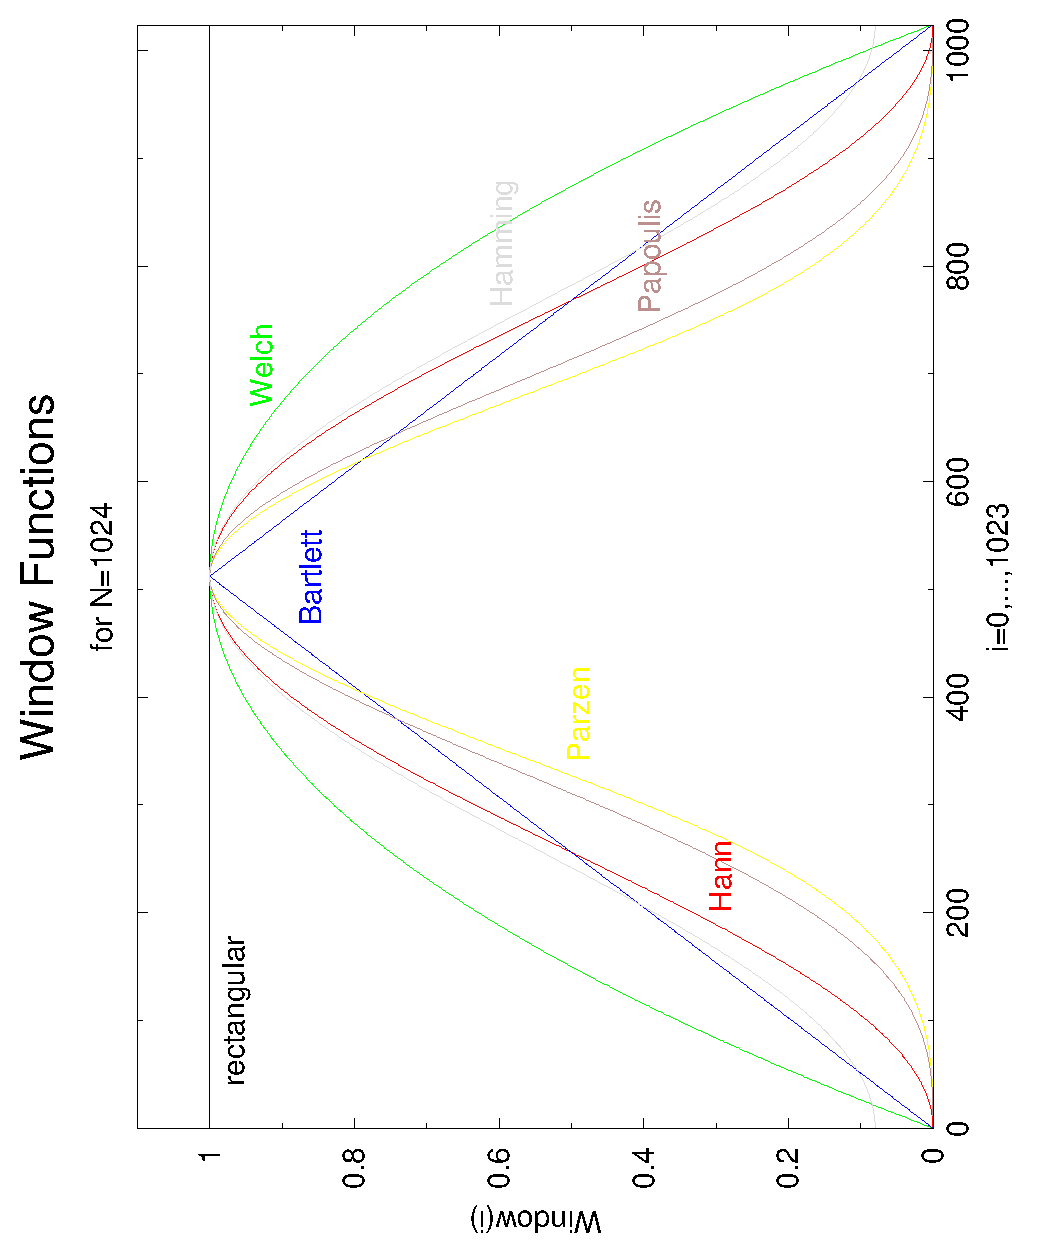
\epsfig{file=Window.eps,angle=-90,width=6in}
\caption{\label{f:window}
The different window functions are shown in different colors, for the
$N=1024$ case. Note that the Hamming window does not vanish at the endpoints.}
\end{figure}

\subsection{References}

% Any references for algorithms, tests, etc.
Definitions of the window functions may be found in {\it Numerical Recipes in C},
the art of scientific computing, Second Edition, eqns. 13.4.13-13.4.15.  Definitions
of the remaining windows can be found in {\it Spectral analysis for physical applications},
by Percival and Walden, in Section 6.11.

\end{document}


